% Number 991
% CAPMA CVPMA Algebra Units 
% Deer stopping, with reaction time - algebraic
% JG

% Watermark
\AddToShipoutPicture*{\BackgroundPic}

\addtocounter {ProbNum} {1}

%\begin{floatingfigure}[r]{.44\textwidth}
%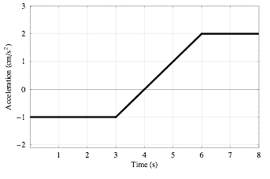
\includegraphics[scale=.95]{/Users/jgates/desktop/latex/pics/agraph1}
%\end{floatingfigure}
 
{\bf \Large{\arabic{ProbNum}}} A car roars down the street, driving ${28~\tfrac{m}{s}}$.  A deer steps into the road 30 meters ahead of the car.  The driver has a .4 second reaction time, after which she slams on the brakes.  The brakes have the ability to stop the car within 1.6 seconds when traveling at this speed (those are pretty great brakes, BTW!).  \bigskip

Two questions: find the car�s acceleration, and�will she stop before hitting the deer?  
\paragraph{}
\noindent
\vfill


%\begin{center}
%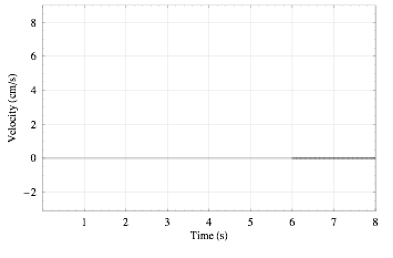
\includegraphics[scale=.7]{/Users/jgates/desktop/latex/pics/vgraph8}
%\end{center}



\newpage